\documentclass{article}

\usepackage{arxiv}

\usepackage[utf8]{inputenc} % allow utf-8 input
\usepackage[T1]{fontenc}    % use 8-bit T1 fonts
\usepackage{hyperref}       % hyperlinks
\usepackage{url}            % simple URL typesetting
\usepackage{booktabs}       % professional-quality tables
\usepackage{amsfonts}       % blackboard math symbols
\usepackage{nicefrac}       % compact symbols for 1/2, etc.
\usepackage{microtype}      % microtypography
\usepackage{lipsum}
\usepackage[T1]{fontenc}
\usepackage{amsmath}
\usepackage{babel}
\usepackage{dirtytalk}
\usepackage{graphicx}
\usepackage{epigraph}
\usepackage{csquotes}
\newtheorem{theorem}{Theorem}

\title{
        Quantifying Immutability in Blockchains\\
        \large The Finney Ratio and Szabo Score
}
\subtitle{}


\author{
        Yaz Khoury \\
        Director of Developer Relations\\
        Ethereum Classic Cooperative\\
        \texttt{yaz@etccooperative.org} \\
}


\begin{document}
\maketitle

\begin{abstract}
Immutability is a term used a lot in blockchain and cryptocurrency development when attempting to analyze the economic interpretation of a network. Designs like the 21 million Bitcoin supply in BTC or incidents like the DAO fork bailout that split the Ethereum community into ETH and ETC are major examples of immutability values determining the ethos of a chain. This research sets out to categorize different features of blockchain immutability and analyze them in three different networks: Bitcoin (BTC), Ethereum (ETH), and Ethereum Classic (ETC). Further in the paper, the Finney Ratio is introduced to help understand how blockchain immutability can be measured over time. The paper then visualizes overall blockchain immutability over time using radar charts as an immutability map. The Szabo Score is then introduced as a tool to score overall mutability over time for each blockchain.

\end{abstract}

\keywords{Immutability \and Blockchain \and Finney Ratio \and Szabo Score \and Bitcoin \and Ethereum Classic}


\section{Introduction}
Cryptocurrency network communities like Bitcoin (BTC), Ethereum (ETH) and Ethereum Classic (ETC) often debate about the concept of immutability and what it means in the context of a blockchain. Bitcoin's white paper\cite{bitcoinpaper}, proposed by Satoshi Nakamoto, introduces a major innovation in Byzantine Fault Tolerance (BFT) problem: It achieves 51\% fault tolerance in what is called Nakamoto Consensus, which is an improvement over other BFT systems. This protects data and ledger immutability up to 51\% of honest nodes on a technical level. However, this paper will show that there are various features of immutability in blockchain networks that still can be broken on the social level. Even if Nakamoto Consensus is still valid, certain social coordinations by network participants can break aspects of blockchain immutability. Another example is the 21 million\cite{bitcoinmailing} Bitcoin supply cap being cited as a source of immutability for the network when it first came online. The adherence to a supply cap is in itself a social level immutability. On a technical level, it is easy to modify the supply cap in Bitcoin, but what protects its value is the adherence to the social contract given in the software origin and the white paper. 

Ethereum\cite{ethpaper} and Ethereum Classic\cite{etcdec} were one chain at a point in time before a hack\cite{daohack} of a famous smart contract known as the DAO (Decentralized Autonomous Organization) allowed the hacker to steal \$50 million dollars at the time. A debate within the Ethereum community turned contentious over whether the community should hard fork to bailout the victims of the DAO hack or preserve ledger immutability. The resulting DAO hardfork\cite{daofork} split the Ethereum community in two with ETH forking to return back the money to those that lost it while Ethereum Classic chosing to run the original chain that resisted the fork. This major event is one of many examples of immutability debates that have occured in the blockchain space.

Currently, immutability is often quantified in the binary sense: is blockchain X immutable or not? However, it's very hard to understand what this binary classification is referring to. Is it referring to a monetary policy, social contracts in a network, or perhaps any changes in the transactions written to a ledger? The applications here are endless and it often confuses stakeholders when trying to properly analyze what it means that a blockchain is immutable.

This paper will attempt to analyze multiple properties common in all blockchain networks and attempt to quantify the immutability of each property. This paper will present ways to do an overall quantification and scoring of each network based on its immutability properties. This research will also visualize the immutability properties of each blockchains so stakeholders can easily understand. This will help network particpants understand how each network differs based on its immutability properties and then understand which network is more immutable than the other. It will also help stakeholders understand how blockchain immutability changes over time.

\section{Immutability Subsystems}
\label{sec:headings}
While measuring blockchain decentralization\cite{quantdecent} through the minimum Nakamoto Coefficient and Gini Coefficient can be quantified more in percentages, immutability on the other hand must be a binary measurement. In other words, a subsystem can either be mutable or immutable. Therefore, this paper will define immutability more as a vector with multiple scalar features in it, each scalar feature with its own value measuring one subsystem.

The immutability variable is defined as the following in Theorem~\ref{th1:theorem}.
\begin{theorem}
Let $i_{subsystem}$ be a variable for immutability,

Where \emph{i} is the immutability variable and
\emph{subsystem }is the sector of the blockchain
whose immutability is being quantified.$ $

Then,
\begin{equation}
    i_{subsystem}\begin{cases}
    \begin{array}
    {cc}
    0 & mutated\\
    1 & immutable
    \end{array}\end{cases} 
    \label{eq1:equation}
\end{equation}
\label{th1:theorem}
\end{theorem}

Here, the \emph{i} variable represents a variable being classified as immutable or mutable, where it refers to a specific subsystem of the blockchain being measured. Various features of the immutability vector can be proposed. This paper aims to focus on eight subsystems of immutability as can be seen in Table~\ref{tab1:table}. All eight of those subsystems will be analyzed and discussed in Section 2. The design of those methods of quantification for immutability allow for further extendability and addition of more subsystems in the future. The eight subsystems will focus on three blockchain networks:
\begin{itemize}
\item Bitcoin
\item Ethereum
\item Ethereum Classic
\end{itemize}

\begin{table}
 \caption{Immutability Subsystems}
  \centering
  \begin{tabular}{ll}
    \toprule
    % \multicolumn{2}{c}{Part}                   \\
    % \cmidrule(r){1-2}
    Number & Subsystem Name      \\
    \midrule
    1 & Monetary Policy \\
    2 & Consensus Mechanism \\
    3 & Hashing Algorithm \\
    4 & Chain State \\
    5 & Reserved State Space \\
    6 & Transaction History \\
    7 & Transaction Finality \\
    8 & Social Contracts \\
    \bottomrule
  \end{tabular}
  \label{tab1:table}
\end{table}

The blockchain subsystems in Table~\ref{tab1:table} can be grouped into an immutability vector as defined in Theorem~\ref{th2:theorem}.

\begin{theorem}
Let $\mathbf{I}$ be the immutability vector,

Where the features of the immutability vector are specified as the following: 
\begin{equation}
   \mathbf{I}=\left[i_{0},i_{1},...,i_{n}\right]
   \label{eq2:equation}
\end{equation}

Where $\mathit{n}$ is the length of the $\mathbf{I}$ immutability vector.

Then, each $i_{subsystem}$ variable inside vector $\mathbf{I}$ represents a unique subsystem of immutability.
\label{th2:theorem}
\end{theorem}

In the following subsections, each subsystem in Table~\ref{tab1:table} will be gone over and analyzed for immutability.

\subsection{Monetary Policy}
Immutability of the Monetary Policy is a measure of the change in the Monetary Policy of the blockchain historically. Examples of monetary policies in blockchains include the 21 million bitcoin supply cap or Ethereum’s infinite supply of Ether. Here, the paper will look at the moment a monetary policy was first described or mentioned and if changes were made to it after. For example, a change in the block issuance number from constant supply to a lower number or a supply cap on the total issued currency units constitutes a change in the monetary policy.

\subsubsection{Bitcoin Monetary Policy}
The question for Bitcoin has always been when was the monetary policy first introduced. The original whitepaper for Bitcoin and the code published by Satoshi Nakaomoto (pre-release version) contain no mention of the 21 million supply cap, around November 2008. It was only in the first-version release in January 2009, a few months later, did Satoshi first mention the 21 million supply cap and references to it in the code.

The question for this research then becomes: which is the right Bitcoin canon, when it was first published in the white paper with the pre-release code or when it first went online in early January 2009? There is a 2 months gap in between where Satoshi Nakamoto first released the Bitcoin white paper and pre-release code and when Satoshi and Hal Finney and others worked on the first version release software, where the supply cap was introduced. A sample of the code written in the first version release\cite{bitcoincode} of the software is shown in the following code block.
\begin{verbatim}
int64 CBlock::GetBlockValue(int64 nFees) const
{
    int64 nSubsidy = 50 * COIN;

    // Subsidy is cut in half every 4 years
    nSubsidy >>= (nBestHeight / 210000);

    return nSubsidy + nFees;
}
\end{verbatim}

In this code block, the block reward is halved approximately every 4 years, or every 210000 blocks. In the pre-release version, the code is not there. The Bitcoin first-version software release in January 2009 contains the following quote by Satoshi, the first ever mention of the 21 million supply cap\cite{bitcoinmailing}:

\begin{displayquote}
"Total circulation will be 21,000,000 coins. It’ll be distributed to network nodes when they make blocks, with the amount cut in half every 4 years." - \textit{Satoshi Nakamoto}
\end{displayquote}

So, this paper will consider the first time the Bitcoin network went online to be on the first version release of the Bitcoin client software. Therefore, Bitcoin’s immutability value for monetary policy is 1, denoted as $i_{monetary policy} = 1$.

However, it is important to note here that Satoshi was not the best programmer and even though he intended there to only be 21 million bitcoins, it actually would continue over 21 million supply due the way C++ language is designed. BIP-42\cite{bip42} intends to set the supply cap to strictly 21 million bitcoins in the year 2214, which by then will violate immutability of monetary policy. So although currently, Bitcoin has a monetary policy value of 1, it will violate it in the year 2214 due to BIP-42.

\subsubsection{Ethereum and Ethereum Classic Monetary Policy}
In the case of Ethereum's white paper\cite{ethpaper}, the monetary policy was an infinite supply with a fixed block reward issuance of 5 ETH for the rest of the chain’s life cycle. However, in Byzantium and Constantinople hard forks, there was a decrease in issuance from 5 to 3 ETH and from 3 to 2 ETH respectively, specifically described in EIP-649\cite{eip649} and EIP-1234\cite{eip1234}. This is clearly a violation of the immutability of monetary policy. While one can argue that Ethereum does not have a monetary policy due to having an infinite supply, the constant issuance of ETH per block for its infinite supply is still a monetary policy. Therefore, Ethereum's monetary policy scores a 0 on immutability, denoted as $i_{monetarypolicy} = 0$.

Ethereum Classic (ETC) follows the same story due to the application of a supply cap on circulating ETC as can be seen in ECIP-1017\cite{ecip1017}. Because Ethereum Classic continues the original chain from the white paper with a resistance to the DAO fork, a change in its monetary policy by issuing a supply cap is a violation of immutability of the monetary policy. Therefore, ETC also scores a 0 on monetary policy, denoted as $i_{monetarypolicy} = 0$.

\subsection{Consensus Mechanism}
Consensus deals with the mechanism of decision-making on the blockchain. The most popular type of consensus is Proof-of-Work\cite{pow}, which is currently found in Bitcoin, Ethereum and Ethereum Classic. Immutability of the consensus mechanism is an important measure of understanding whether a blockchain is modifying its mechanism in the future.

For example, if Ethereum moves from Proof-of-Work to Programmatic Proof-of-Work (ProgPoW)\cite{progpow} or to Proof-of-Stake, it breaks the immutability value for consensus mechanism. What's more interesting about Ethereum is ETH 2.0 plans. If the plan for ETH 2.0 is to not share state with ETH1X (current chain), then technically ETH2 becomes its own network with own state and monetary policy and consensus mechanism, starting fresh from scratch. If however it shares the state with current ETH1X, then it will be violating immutability of the consensus mechanism by moving directly to Proof-of-Stake. Analysis of ETH1X to ETH2.0 is outside the scope of this research paper.

Currently, all three coins (ETC, BTC, and ETH) have always been on Proof-of-Work consensus, so the value for each of them is denoted as: $i_{consensusmechanism} = 1$.

\subsection{Hashing Algorithm}

Hashing algorithms refer to the tools used to measure consensus mechanism. For example, most Proof-of-Work chains like BTC use Hashcash\cite{hashcash} based on SHA-256 algorithm while and ETH/ETC use Ethash\cite{ethash} that is based on Keccak-256. If at any time in the future, any of those chains switch the hashing algorithm to be SHA-3 or some other algorithm, then it violates immutability of the hashing algorithm.

This can be useful to do if for instance SHA-256 is broken in the future and the security of all those chains relies on having a harder to break hashing algorithm. By then, despite breaking immutability in that category by moving to a new hashing algorithm, it actually improves security. It is a trade-off of security vs. maximum immutability.

For now, though, all three chains will receive a score of 1, denoted as: $i_{hashingalgorithm} = 1$.

\subsection{Chain State}

The immutability of the state set is the assumption that the state never gets irregularly modified outside of its regular change. In other words, if we assume the state of the blockchain is \textbf{S}, where \textbf{S} is constantly being updated and modified regularly with each block, any irregular modification of \textbf{S} would denote a value \textbf{S'} such as \textbf{S'} is an irregular State set. What we define as irregular state change is anything that affects the transaction history and finality of the ledger in any way.

To date, only one chain has made an irregular state change, resulting in an \textbf{S'} prime: Ethereum during the DAO Hard Fork\cite{daofork}. The irregular state change allowed for a bailout of stolen money from the DAO hacker, which has modified the state to result in \textbf{S'}.

Chain State can be written in the following Theorem:
\begin{theorem}
Let $S_{t}$ denote a blockchain state,

Where the state $S$ being regularly changed through time $t$ is
$S_{t}$

Then,
\begin{equation}
    S_{t-1}\Rightarrow S_{t} 
\end{equation}
\begin{equation}
    S_{t-1}\Rightarrow S_{t}'
\end{equation}

Where (3) is a regular state change denoted with $S_{t}$ and (4) is an irregular state change denoted with $S$$_{t}$$'$.
\end{theorem}

Using this definition, the immutability values for ETC and BTC are 1, denoted as $i_{chain state} = 1$ while ETH is 0, denoted as $i_{chain state} = 0$.

\subsection{Reserved State Space}
Reserved State Space is a measure of empty addresses that are reserved for future modifications on the blockchain to allow for the addition of new features. For example, when one adds in op-codes for Solidity like REVERT on Byzantium Hardfork\cite{byzantium} for Ethereum or the Atlantis Hardfork\cite{atlantis} for Ethereum Classic, they are modifying the reserved state space which was initially empty.

This category is important to note that the modification of empty reserved state space follows its intended design and even if there has been a new addition of op-codes that break immutability here, it is acceptable because that is the whole point of using reserved state space. Currently, Bitcoin has a 0 for no modification of reserved state space because Bitcoin added its first new op-code in December 2015 with BIP-65\cite{bip65}. Ethereum, having implemented Byzantium and Constantinople hardforks which added several new op-codes, breaks immutability in this category. Ethereum Classic having implemented the Atlantis Hardfork, also violates immutability in the reserved state space category.

So, here, ETC, ETH and BTC all get a value of 0, denoted as $i_{reserved state space} = 0$.

\subsection{Transaction History}
Ethereum’s bailout of the DAO token holders who lost their ETH during the DAO hack isn’t a violation of transaction history on the ledger because the original transaction by the DAO hacker to steal the ETH was not modified in the future by the DAO fork. Instead, what the DAO fork introduced was an irregular state change, as discussed in the previous Section 2.4.

Therefore, in this category, historically, neither of the three chains every experienced a violation of transaction history immutability. So, each chain gets a score of 1, denoted as $i_{transaction history} = 1$.

\subsection{Transaction Finality}
In transaction finality, this paper looks at whether a transaction that enters the blockchain after some confirmations is final. Since blockchains are probabilistic and the more confirmations a transaction has, the more it is final, the measure becomes one of what constitutes a good amount of confirmations.

If one decides a confirmation of 1 block for each chain, we are in trouble because sometimes 51\% attacks and blockchain reorganizations\cite{reorg} happen. Reorganizations or reorgs can happen if say there is a delay in network propagation from miners in China, which means a transaction that is added to a block mined by someone in America might not be final if for example a miner in China has mined a longer chain but has a delay in communicating with the rest of the network. By the time they do, their chain becomes the longer chain and the other transactions will have to be re-added to the network. Therefore, transaction finality on one block confirmation would result in a 0 for all chains and is an unrealistic way of looking at immutability of transaction finality.

It is important to understand that due to 51\% weakness of Proof-of-Work chains, waiting for longer confirmations is the only way to probabilistically reach transaction finality. In the events of the 51\% attack on Ethereum Classic\cite{51per} with a double-spend attack on two exchanges, exchanges were waiting for shorter block confirmations than the economic security of 6 bitcoin blocks\cite{bitconf}. No other transaction was lost in the process, but the finality at the moment was threatened on the exchange side.

The solution was longer confirmation times. This paper will use the Coinbase metric for confirmation times\cite{confirmations} that are fit for each chain, which then results in BTC, ETH, and ETC all having a score of 1, denoted as $i_{transaction finality} = 1$. To further illustrate the point of how longer confirmation times improve transaction finality, observe the early interactions between Satoshi Nakamoto and Hal Finney\cite{maillist} on the following quote.

\begin{displayquote}
The transaction in whichever branch ends up getting ahead becomes the valid one, the other is invalid. If someone tries to double spend like that, one and only one spend will always become valid, the others invalid. Receivers of transactions will normally need to hold transactions for perhaps an hour or more to allow time for this kind of possibility to be resolved. They can still re-spend the coins immediately, but they should wait before taking an action such as shipping goods. — \textit{Satoshi Nakamoto}
\end{displayquote}

\subsection{Social Contracts}

Social Contracts relates to any rules that a user acknowledges before using the blockchain. A violation of social contracts is a change in immutability. Many examples of social contracts exist, such as "Code is Law", "21 million", or "No Dev Block Rewards", but here, the paper will use the example of private and public key rules. The rule of blockchains is that only the owners of the private keys can transact from the address and the account. So, if a user does not own the private key of an account on the blockchain with say 1 million ETH, they can’t move those ETH around.

This is why it is important that Satoshi’s address on Bitcoin has 1 million BTC that has not been moved. It’s also why Craig Wright can’t prove he is Satoshi because he does not own the private key for the address that is known to belong to Satoshi. In the case of the DAO hard fork, a violation of social contract has taken place with the bailout of stolen funds on a new forked network by Ethereum, which makes ETH mutable in this category and is therefore assigned a value of 0, denoted as $i_{social contract} = 0$.

Ethereum Classic was a rejection of the DAO hard fork and therefore still maintains on the social layer the social contract, making it still a 1. However, ECIP-1015\cite{ecip1015} which modified the gas costs on Ethereum Classic did violate the Social Contract on block 2,463,000, since a modification gas costs violate the immutability of the network promised to network participants to deploy their contracts or to transact on the chain. Therefore, ETC has a value of 0 in this category. There has never been historically a bailout in the history of Bitcoin, even during the Mt. Gox Hack, so it retains a value of 1, denoted as $i_{social contract} = 1$.

\section{The Finney Ratio and Immutability Maps}
This paper has done the preliminary analysis of the immutability features in Section 2. They are summarized in Table~\ref{tab2:table}. Binary values for each immutability variable gives an immediate picture of whether or not there is a mutation in one of the features. While Table~\ref{tab2:table} provides a quick way to measure blockchain immutability, this paper is also interested in measuring blockchain immutability over. 

The benefit of using time is that stakeholders can actually see how long each feature of a blockchain stays immutable before there is a violation in immutability. This paper will measure time passing in blockchain via block numbers. This paper proposes the Finney Ratio, denoted as $R_{finney}$, for measuring time passage in blockchain with mutated features, as defined in Theorem~\ref{th4:theorem}

\begin{table}
 \caption{Immutability Vectors Table}
  \centering
  \begin{tabular}{llll}
    \toprule
    \cmidrule(r){1-2}
    Immutability Features     & Bitcoin     & Ethereum & Ethereum Classic \\
    \midrule
    Monetary Policy & 1 & 0 & 0     \\
    Consensus Mechanism & 1 & 1 & 1     \\
    Hashing Algorithm & 1 & 1 & 1     \\
    Chain State & 1 & 0 & 1     \\
    Reserved State Space & 0 & 0 & 0     \\
    Transaction History & 1 & 1 & 1     \\
    Transaction Finality & 1 & 1 & 1     \\
    Social Contract & 1 & 0 & 0     \\
    \bottomrule
  \end{tabular}
  \label{tab2:table}
\end{table}

\begin{theorem}
Let $B_{mutate}$ equal the block number where the violation in immutability occurs,

Let $B_{height}$ equal the block number of the height or latest block in the blockchain.

Then, the Finney Ratio is: 
\begin{equation}
    R_{finney}=\frac{B_{mutate}}{B_{height}}
\end{equation} 

Which is the ratio between the mutated block number and the latest block number.
\label{th4:theorem}
\end{theorem}

Here, the Finney Ratio applies to any of the immutability variables that have a 0 value. So, for all variables in immutability vector \textbf{I}, the 0 is replaced with the correct Finney Ratio $R_{finney}$. This gives the ratio of when the mutation occurs (as measured by block number it occurs on) by the latest block value. For the calculations for this paper, the following latest block numbers $B_{height}$ (latest) will be used in the calculations for each chain:

\begin{itemize}
\item \textbf{Bitcoin}: Block 600762
\item \textbf{Ethereum}: Block 8798811
\item \textbf{Ethereum Classic}: Block 9044480
\end{itemize}

\subsection{Ethereum Finney Ratio}
Ethereum’s violation of Monetary Policy immutability happens around the Byzantium Hard Fork where there was a reduction in reward at block number 4,370,000\cite{eip649}. It is also the same block where the new op-codes were added\cite{byzantium}, violating Reserved State Space category of immutability. So, the Finney Ratio for those two categories is $R_{finney} = 4.37 / 8.798811 = 0.4966$.

In regards to the other violations, both the violation in Social Contract and Chain State happen on the DAO Fork at block number 1,920,000\cite{daofork}. So, the Finney Ratio for those two categories is $R_{finney} = 1.92 / 8.798811 = 0.2182$. Table~\ref{tab3:table} groups the Finney Ratios back into the immutability vector for Ethereum. 

Table~\ref{tab3:table} can now be plotted as radar chart that will be called an immutability map for this paper where immutability over time can be visualized, as can be seen in Figure~\ref{fig:fig1}. Here, the effects of the DAO in early penalization of Ethereum can be observed, with the larger growth in the chain pushing the Chain State and Social Contract closer to 0 as time passes on. One can also observe the effects of Byzantium Hard Fork on the network.

\begin{table}
 \caption{Ethereum Finney Ratio}
  \centering
  \begin{tabular}{ll}
    \toprule
    \cmidrule(r){1-2}
    Immutability Features & Ethereum \\
    \midrule
    Monetary Policy & 0.4966     \\
    Consensus Mechanism & 1     \\
    Hashing Algorithm & 1     \\
    Chain State & 0.2182     \\
    Reserved State Space & 0.4966     \\
    Transaction History & 1     \\
    Transaction Finality & 1     \\
    Social Contract & 0.2182     \\
    \bottomrule
  \end{tabular}
  \label{tab3:table}
\end{table}

\begin{figure}
  \centering
  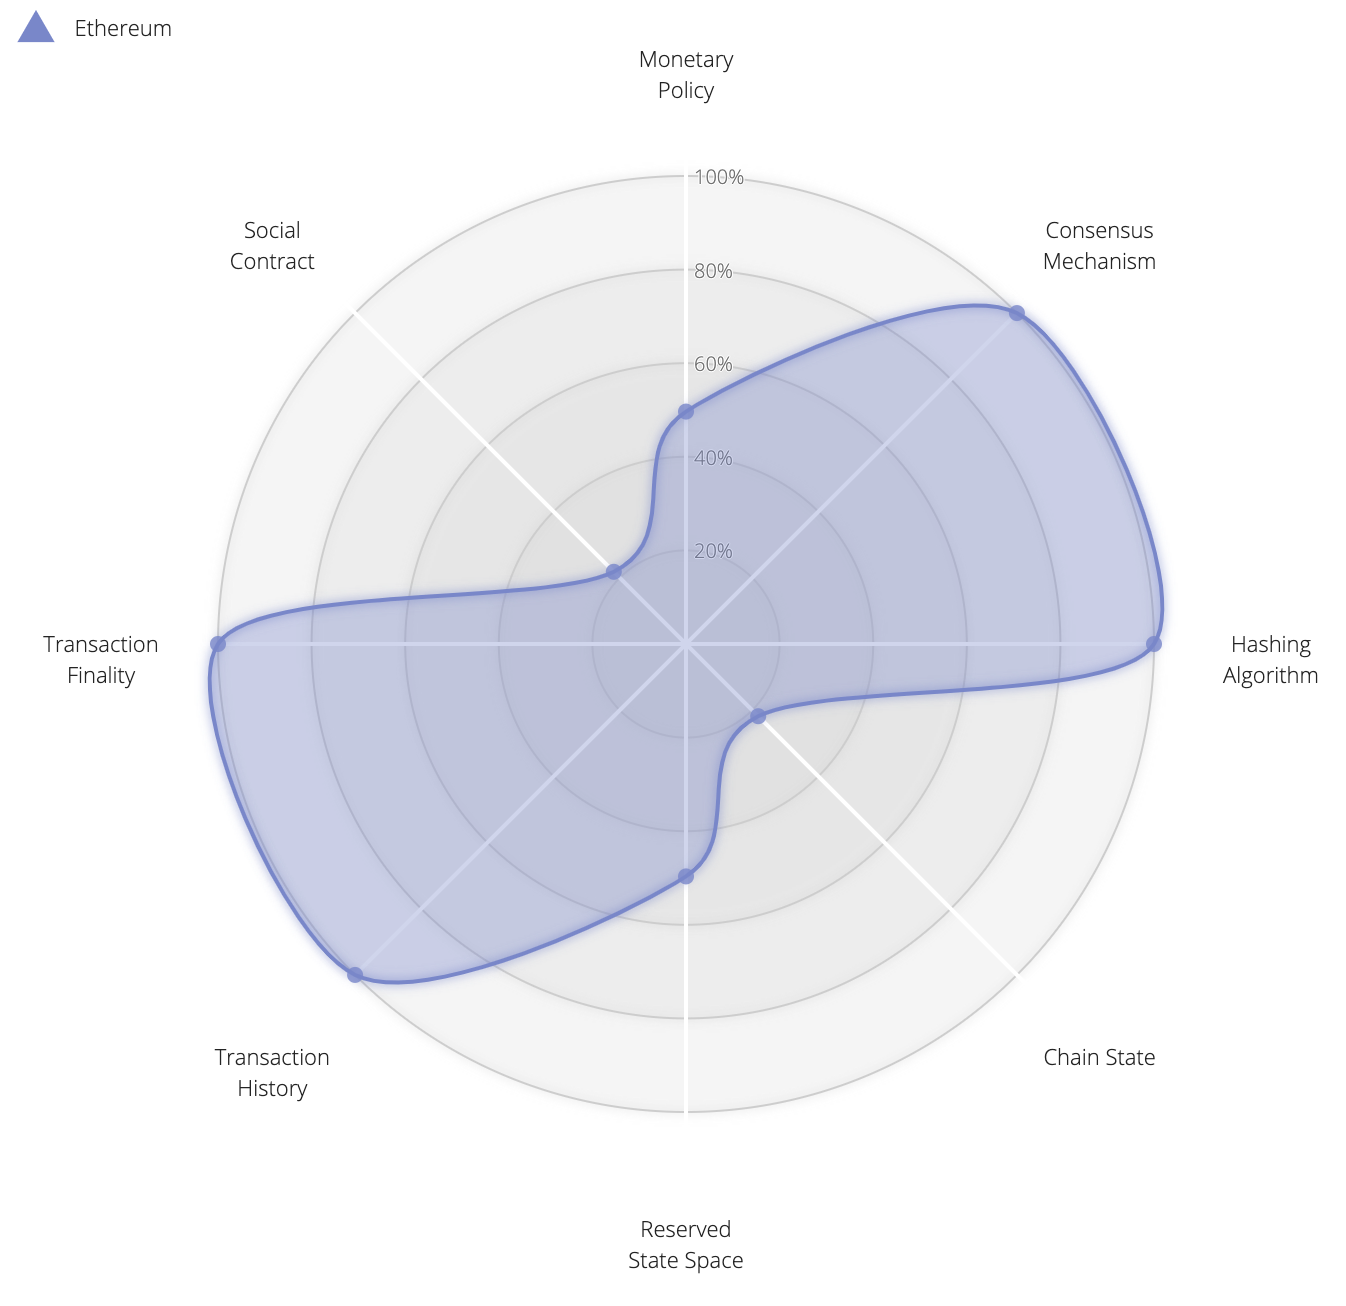
\includegraphics[width=12cm]{eth.png}
  \caption{Ethereum Immutability Map}
  \label{fig:fig1}
\end{figure}

\subsection{Ethereum Classic Finney Ratio}
In Ethereum Classic, three violations happened, the Monetary Policy breaking in immutability which happens at block 5,000,000, the Social Contract violation back at block 2,463,000 for ECIP-1015, and the Atlantis Hardfork at block 8,772,000 which is a violation of Reserved State Space immutability. This will result in a Finney Ratio of $R_{finney} = 0.5528$ for Monetary Policy, a Finney Ratio of $R_{finney} = 0.27232$ for Social Contract, and one of $R_{finney} = 0.96987$ for Reserved State Space. Table~\ref{tab4:table} highlights the values calculated for Ethereum Classic's Finney ratios. An immutability map of the Finney Ratios is plotted in Figure~\ref{fig:fig2}.

\begin{table}
 \caption{Ethereum Classic Finney Ratio}
  \centering
  \begin{tabular}{ll}
    \toprule
    \cmidrule(r){1-2}
    Immutability Features & Ethereum Classic \\
    \midrule
    Monetary Policy & 0.5528     \\
    Consensus Mechanism & 1     \\
    Hashing Algorithm & 1     \\
    Chain State & 1     \\
    Reserved State Space & 0.96987     \\
    Transaction History & 1     \\
    Transaction Finality & 1     \\
    Social Contract & 0.27232     \\
    \bottomrule
  \end{tabular}
  \label{tab4:table}
\end{table}

\begin{figure}
  \centering
  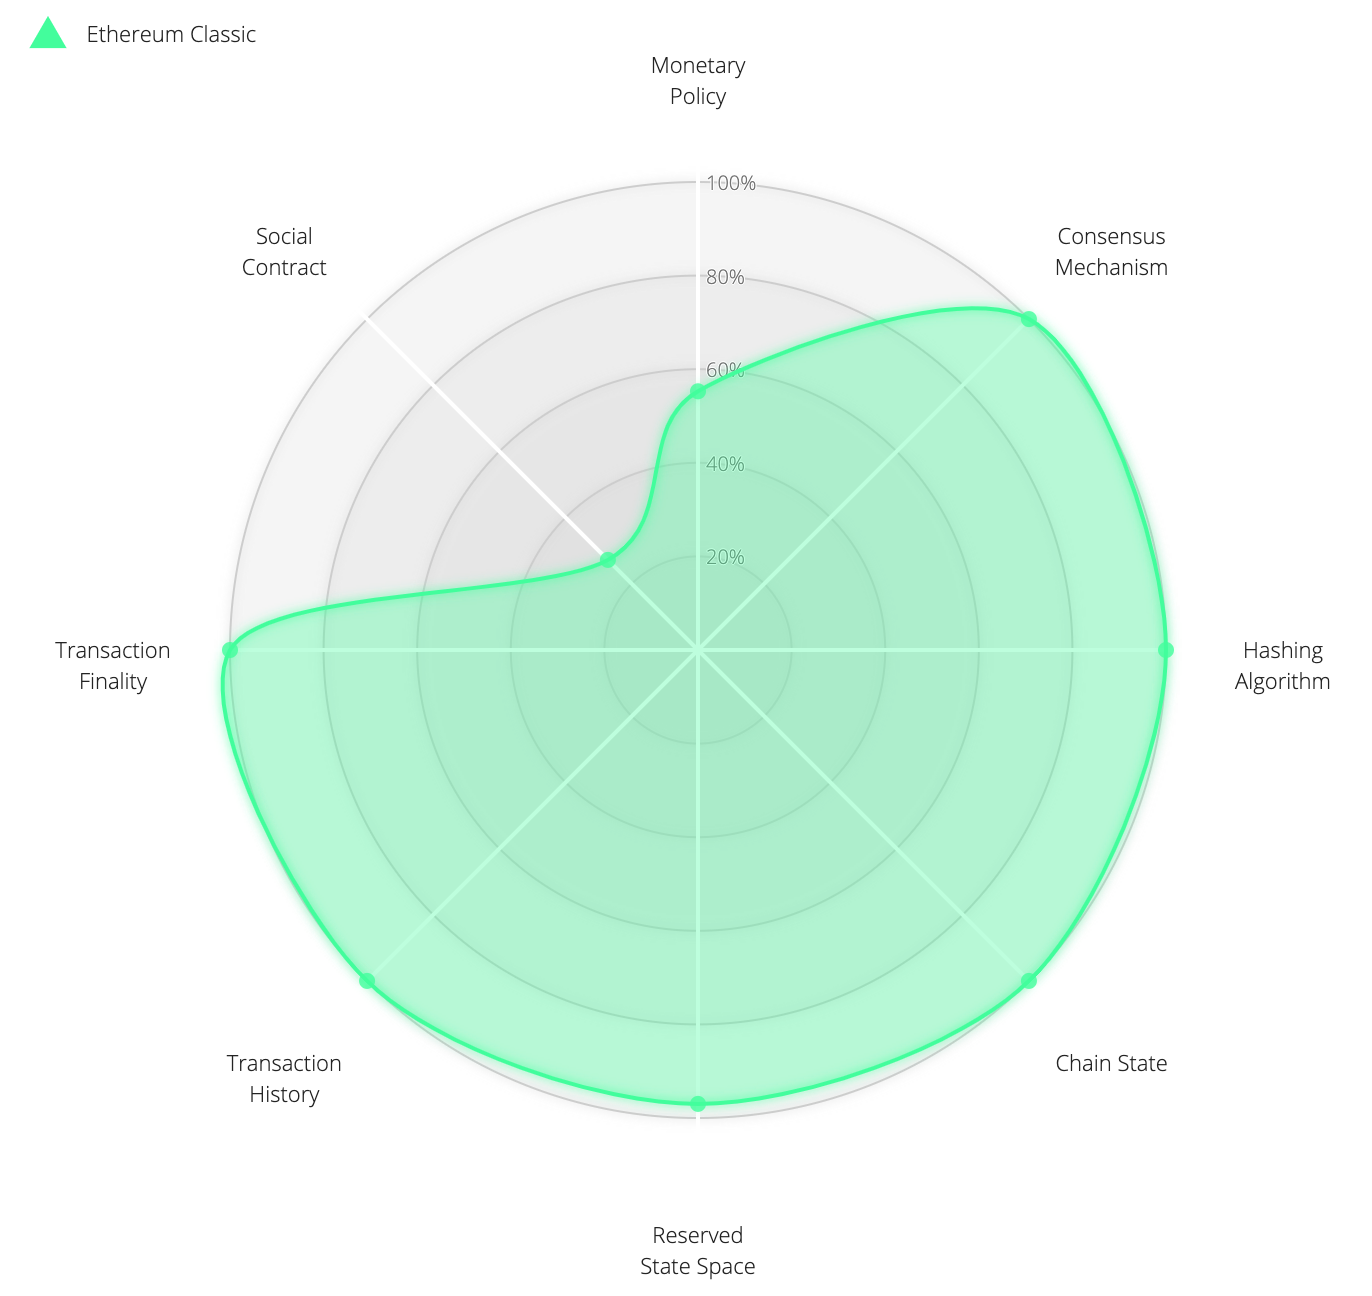
\includegraphics[width=12cm]{etc.png}
  \caption{Ethereum Classic Immutability Map}
  \label{fig:fig2}
\end{figure}

The violation in Monetary policy for ETC has a Finney ratio of 0.5528, which is close to the Finney ratio of 0.4966 for ETH’s violation in monetary policy immutability, indicating the periods where both network's violations have occurred are close to one another.

\subsection{Bitcoin Finney Ratio}

For Bitcoin, the violation of Reserved State Space happens around December 2015 with the implementation of BIP-65 for adding a new op-code. No information about when in December 2015 has BIP-65 been activated, or rather at which specific block, due to it being a User Activated Soft Fork (UASF). This paper instead takes an estimate based on the minimum and maximum block number for December 2015 via the timestamp of the block being included in the ledger. Then, the average of both minimum and maximum blocks  give the approximate block number.

\begin{itemize}
\item 386,270 is Minimum Block number on December 2015
\item 391,150 is Maximum Block number on December 2015
\end{itemize}
Average Block Number for BIP-65 is 388,710. So, the Finney Ratio for Reserved State Space is $R_{finney} = 0.647$. Table~\ref{tab5:table} shows the updated immutability vector values with the Finney ratio. A plot of the Bitcoin immutability map is shown on Figure~\ref{fig:fig3}.

\begin{table}
 \caption{Bitcoin Finney Ratio}
  \centering
  \begin{tabular}{ll}
    \toprule
    \cmidrule(r){1-2}
    Immutability Features & Bitcoin \\
    \midrule
    Monetary Policy & 1     \\
    Consensus Mechanism & 1     \\
    Hashing Algorithm & 1     \\
    Chain State & 1     \\
    Reserved State Space & 0.647     \\
    Transaction History & 1     \\
    Transaction Finality & 1     \\
    Social Contract & 1     \\
    \bottomrule
  \end{tabular}
  \label{tab5:table}
\end{table}

\begin{figure}
  \centering
  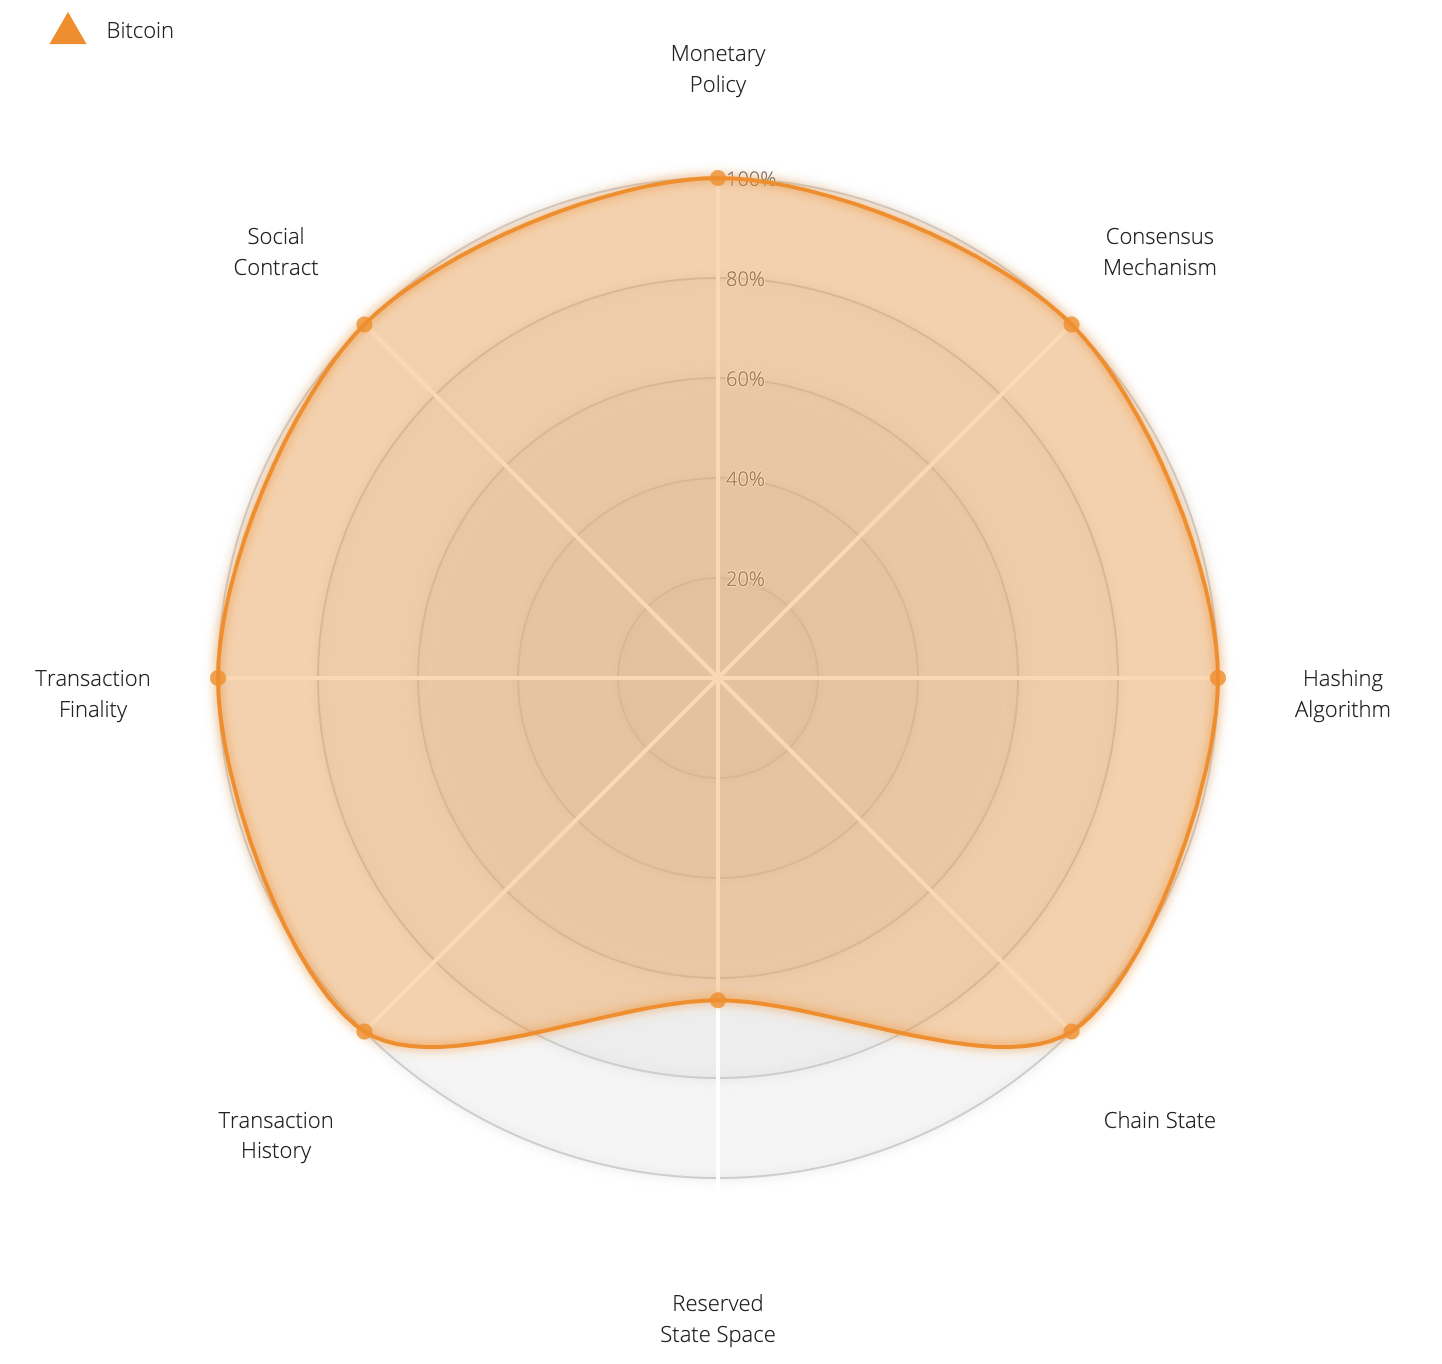
\includegraphics[width=12cm]{btc.png}
  \caption{Bitcoin Immutability Map}
  \label{fig:fig3}
\end{figure}

What’s the benefit of calculating the Finney ratio for each violation in immutability in the Immutability vector? It helps stakeholders understand the timelines of blockchain immutability better when they can see how long a blockchain’s features preserve immutability through time. One property of Finney Ratio given a long enough timeline, the Finney Ratio $R_{Finney}$  approaches zero. The longer a blockchain preserves immutability in each of its features, the larger the immutability map.

In the case of Bitcoin, it is going to maintain a great area of immutability until BIP-42 is implemented around the year 2214 whereafter, the violation in Monetary Policy value happens, as covered in Section 2.1.1. In the following section, the paper will provide a score of immutability for each blockchain network.

\section{The Szabo Score}

In order to quantify the immutability maps plotted to a score number, this paper proposes using the Szabo Score. The Szabo Score is simply using the entropy formula to quantify a blockchain’s immutability. It is specified in Theorem 5. Why use entropy here to measure mutations in blockchain over time? In information theory, entropy measures the unpredictability of the state. 

If a highly probable event happens, it gives no new information about it since it’s expected to happen. Also, if a lower probable event happens, it gives a lot of more information of when it occurs. So, in entropy, flipping a dice has a higher value because of the low probability of each dice value than say flipping a coin.

This paper replaces probability with immutability as measured via the Finney Ratio. Here, if a Finney Ratio is 1 for each value of the immutability variables, it gives no new information as it will always be a 1, and thus, fully immutable. The entropy value of a fully immutable vector (all values are 1) is 0. The interest lies in variables where there is a violation of immutability, or a mutation, and pushing the Finney Ratio towards 0 over time. Here, over time, the dropping in Finney Ratio for one of the variables does increase the mutability or Szabo Score. It allows stakeholders to gauge how a violation in immutability in a blockchain leads to more uncertainty over time.

The Shannon Entropy\cite{entropy} formula can be rewritten in terms of the Szabo Score as follows:

\begin{theorem}
Let $S_{szabo}$ denote the Szabo score,

Let $R$$_{finney}$ denote the Finney ratio,

Where $I_{i}$ denotes all Finney ratios $i$ in the Immutability
Vector $\emph{I}$.

Then,

Szabo score can be written as follows:

\begin{equation}
    S_{szabo}=-\sum_{i}I_{i}\log_{10}I_{i}
\end{equation}
\end{theorem}

Szabo Score is measuring on a base of 10 of the logarithm because it is concerned with decimals and not binary points. Given the vector values of each chain in the previous tables where the 0s are replaced with their Finney Ratios, the Szabo Scores of each chain can be calculated as shown in Table~\ref{tab6:table}.

\begin{table}
 \caption{Szabo Score Table}
  \centering
  \begin{tabular}{llll}
    \toprule
    \cmidrule(r){1-2}
    Blockchain & Szabo Score \\
    \midrule
    Bitcoin & 0.1223 \\
    Ethereum & 0.5904 \\
    Ethereum Classic & 0.3090 \\
    \bottomrule
  \end{tabular}
  \label{tab6:table}
\end{table}

Here, it can be seen that the higher the Szabo Score, the less immutable a blockchain is over time, and therefore the more mutation is in a blockchain. The more time passes after a blockchain violates one of its immutability variables, the higher the Szabo score climbs, decreasing its immutability. Bitcoin in Table~\ref{tab6:table} above has the lowest Szabo Score, therefore the highest immutability. Ethereum Classic has a higher immutability than Ethereum due to its lower Szabo Score. 

A good way to measure the immutability of blockchains is to take the Szabo Score (entropy of the immutability vector with mutable values of 0 replaced by their Finney Ratio) and the minimum Finney Ratio (ratio of the first break in the immutability of a blockchain feature) to be able to understand blockchain immutability and their timelines better.

\section{Conclusions}

One of the most important aims of this research was to allow stakeholders to visualize immutability in blockchains over times. Having tools like the Finney Ratio, Immutability Maps and the Szabo Score help quantify and analyze blockchain immutability at a deeper level. Being able to do quantify immutability in a coherent manner that helps stakeholders understand the implications of blockchain immutability allows for decision making on what aspects of immutability are important to a community’s values.

For example, a break in SHA-256 algorithms and an network upgrade to SHA-3 algorithm violates the Hashing Algorithm category of immutability but improves security. This an important trade-off a blockchain community must make to preserve immutability of its social contract but sacrifice immutability of hashing algorithm. Moving from Proof-of-Work to Proof-of-Stake violates Consensus Mechanism of immutability but improves scalability in the long term. In the case of ETH 2.0, that is an acceptable goal, the trading of immutability and higher security for scalability and speed. 

Adding new op-codes violates Reserved State Space but extends blockchain functionality over the long term by improving the Turing-completeness properties of blockchains. The aim of this paper was to not be subjective to which features of immutability were more important than others since that was political and local to the network's underlying social layer. What can be done in future research is categorizing immutability features based on technical maintenance vs. socio-economic immutability properties. In this research, eight subsystems or features of immutability were considered and analyzed. 

However, the immutability vector is not limited to just eight. More properties and features can be considered and added to the vector for analysis. For example, one can add backward-compatibility as a feature of immutability. If new changes added to blockchains in a hardfork break backward-compatibility of existing contracts, that violates this immutability.

While technical immutability of transactions is preserved via Nakamoto Consensus of following the longest chain in Proof-of-Work networks, it is important to consider that all those different subsystems that affect a blockchain’s immutability happen on the social layer. On the social layer, stakeholders can propose a hard fork to add a supply cap or remove restrictions and caps. Stakeholders can implement an irregular state change to return back people’s money or they can add new op-codes. 

They can break agreed-upon social contracts or add new ones. The technical probabilistic immutability of Nakamoto Consensus that protects networks up to 51\% fault tolerance is not enough. Social layer quantification of immutability is important to ensure stakeholders understand the risks in modifying immutability properties of a blockchain and adding more complexity instead of minimizing trust. 

In Sections 3 and Section 4 of quantifying and visualizing the immutability of the different blockchain networks, Bitcoin scores the highest on immutability. It has the lowest Szabo Score on mutability, making it the most resilient of all networks to changes. What is also interesting about Bitcoin is that it has the longest timeline of the three networks analyzed yet its still the most resilient to change. 

One aspect of Bitcoin's immutability was not categorized for this research: the inflation bug. The categorization of this bug might fall under "Transaction Malleability" or potentially some other feature if a pattern is found for this bug in other networks.

Another interesting property to highlight is the delta block time and its relation to immutability over time. The higher the delta block time between two blocks, the more immutable it is over time according to the model proposed in this paper due to the fact that the Finney Ratio for such a network slowly decreases vs. a network with faster delta block time. There are plenty of arguments to support longer block time vs shorter block time in Proof-of-Work networks. A relationship to immutability can potentially add an extra signal to stakeholders considering delta block time design. Bitcoin scoring the highest in immutability due to its low Szabo Score has block times that average around 10 minutes, while Ethereum and Ethereum Classic have block times that average around 15 seconds.

One final remark on the methodology used in this research paper is the ability to predict future immutability. If a stakeholder knows what new changes will occur on a blockchain at a specific hardfork in the future, they can plot a future immutability map and quantify immutability at a block height far in the future while accounting for any violations that will occur on a specific hard fork block. This allows one to understand how future hard forks can change the immutability and behavior of blockchain networks. The important thing to note, however, is that immutability is about trade-offs in the end and each blockchain community would then need to decide which trade-offs and features of immutability are worth preserving.

\bibliographystyle{unsrt}  
\bibliography{references}
\end{document}
